\documentclass[12pt,addpoints]{repaso}
\grado{2}
\nivel{Secundaria}
\cicloescolar{2024-2025}
\materia{Ciencias y Tecnología: Física \normalfont \color{darkgray} \\[-0.2em] \small con adecuación curricular.}
\unidad{1}
\title{Practica la Unidad}
\aprendizajes{\footnotesize%
\item Identifica problemas de la vida cotidiana y plantea soluciones.\\[-1.2em]
\item Conoce y caracteriza el pensamiento científico para plantearse y resolver problemas en la escuela y su cotidianidad.\\[-1.2em]
\item Valora la influencia del conocimiento científico y tecnológico en la sociedad actual.\\[-1.2em]
\item Identifica las unidades de medición que se ocupan en su entorno escolar, familiar y en su comunidad.\\[-1.2em]
\item Identifica cuáles son, cómo se definen y cuál es la simbología de las unidades básicas y derivadas del Sistema Internacional de Unidades.\\[-1.2em]
\item Realiza conversiones con los múltiplos y submúltiplos al referirse a una magnitud.\\[-1.2em]
\item Conoce los instrumentos de medición, materiales, sus propiedades y características.\\[-1.2em]
\item Relaciona e interpreta las teorías sobre estructura de la materia, a partir de los modelos atómicos y de partículas y los fenómenos que les dieron origen.\\[-1.2em]
\item Explora algunos avances recientes en la comprensión de la constitución de la materia y reconoce el proceso histórico de construcción de nuevas teorías.\\[-1.2em]
\item Experimenta e interpreta los modelos atómicos y de partículas al proponer hipótesis que expliquen los tres estados de la materia, sus propiedades físicas como la temperatura de fusión, ebullición, densidad, entre otros.\\[-1.2em]
\item Interpreta la temperatura y el equilibrio térmico con base en el modelo de partículas.\\[-1.2em]
}
\author{Melchor Pinto, J.C.}
\begin{document}\vfill
\INFO\afterpage{\blankpage}%
% \begin{multicols}{2}
	\tableofcontents
% \end{multicols}
\newpage
\begin{questions}\large

	\addcontentsline{toc}{section}{Unidad 1}
	\section*{Unidad 1}
	
    \questionboxed[10]{Selecciona la respuesta correcta:

		\begin{parts}

			\part Son características de los sólidos, excepto:
			\begin{choices}
				\choice Sin forma definida
				\choice	No se pueden comprimir
				\choice	Cohesión entre sus partículas alta
				\choice	Volumen definido
			\end{choices}

			\part La _______ ocurre cuando la temperatura de un sólido aumenta, haciendo que aumente su volumen.
			\begin{choices}
				\choice Dilatación
				\choice	Evaporación
				\choice	Fusión
				\choice	Condensación
			\end{choices}

			\part ¿Qué es la cohesión?
			\begin{choices}
				\choice La fuerza de repulsión que existe entre las partículas de una misma sustancia.
				\choice	La fuerza de atracción que existe entre las partículas de una misma sustancia.
				\choice	La fuerza de atracción que existe entre dos partículas con carga opuesta.
				\choice	La fuerza de repulsión que existe entre dos partículas con la misma carga.
			\end{choices}

			\part Las siguientes son características de los gases, excepto:
			\begin{choices}
				\choice Se pueden comprimir.
				\choice	Sus partículas están separadas en unas más simples con carga eléctrica.
				\choice	No tienen forma definida.
				\choice	No tienen volumen definido.
			\end{choices}

			\part Para comprender los estados de agregación de la materia se puede utilizar el modelo cinético de partículas, considerando...
		
            \begin{choices}
				\choice la cohesión y el tipo de sustancia que es.
				\choice	la cohesión y la energía de las partículas.
				\choice	la densidad y la temperatura.
				\choice	la energía de las partículas y su temperatura.
			\end{choices}

			\part ¿Qué fenómeno se observa cuando se empaña el vidrio de un auto?
			
            \begin{choices}
				\choice Solidificación
				\choice	Fusión
				\choice	Condensación
				\choice	Evaporación
			\end{choices}

			\part ¿A qué se debe que el agua se evapore a 100 $°$C al nivel del mar, pero a 70 $°$C a 8,848 metros sobre el nivel del mar?
			\begin{choices}
				\choice A la presión
				\choice	A la temperatura
				\choice	A la altitud
				\choice	Al tipo de agua
			\end{choices}

			\part Cuando se aplica alcohol a una herida y este se convierte en su forma gaseosa rápidamente, ¿qué cambio de estado ocurre?
			\begin{choices}
				\choice Ionización
				\choice	Sublimación
				\choice	Evaporación
				\choice	Fusión
			\end{choices}

			\part Cuando un relámpago atraviesa la atmósfera, en su camino se forma plasma debido a la gran cantidad de energía que absorben las moléculas de la atmósfera. ¿Qué cambio de estado ocurre en esa situación?
			\begin{choices}
				\choice Deposición
				\choice	Ionización
				\choice	Fusión
				\choice	Condensación
			\end{choices}
		\end{parts}
	}

	\questionboxed[10]{Selecciona la respuesta correcta:

		\begin{parts}
			\part Son cambios de estado excepto:
			
            \begin{choices}
				\choice Ionización
				\choice	Liofilización
				\choice	Sublimación
				\choice	Condensación
			\end{choices}

			\part La energía cinética promedio de las partículas depende de...
		
            \begin{choices}
				\choice la presión.
				\choice	la humedad.
				\choice	la temperatura.
				\choice	la cantidad de partículas.
			\end{choices}

			\part ¿Cómo es el movimiento de las partículas entre colisiones?
			\begin{choices}
				\choice En línea recta
				\choice	En órbitas circulares
				\choice	Errático
				\choice	Uniformemente acelerado
			\end{choices}

			\part El volumen de un gas está conformado principalmente por...
			\begin{choices}
				\choice agua.
				\choice	vacío.
				\choice	partículas.
				\choice	aire.
			\end{choices}

			\part ¿Qué implica que aumente la temperatura de un gas para las partículas que lo conforman?
			\begin{choices}
				\choice Aumenta su energía cinética.
				\choice	Disminuye el número de colisiones entre partículas.
				\choice	La cantidad de vacío disminuye.
				\choice	Se mueven más lentamente.
			\end{choices}

			\part ¿Qué se necesita tomar en cuenta para poder aplicar el modelo cinético de partículas a los líquidos y los gases?
			\begin{choices}
				\choice El estado de agregación.
				\choice	La cantidad de materia presente.
				\choice	La forma del recipiente que los contiene.
				\choice	Las fuerzas de atracción entre partículas.
			\end{choices}

			\part La energía cinética promedio de las partículas depende de...
			\begin{choices}
				\choice la presión.
				\choice	la cantidad de partículas.
				\choice	la humedad.
				\choice	la temperatura.
			\end{choices}

			\part ¿Cómo es el movimiento de las partículas entre colisiones?
			\begin{choices}
				\choice Uniformemente acelerado
				\choice	Errático
				\choice	En línea recta
				\choice	En órbitas circulares
			\end{choices}

			\part Según el modelo cinético de partículas, ¿cuál de las siguientes no es una característica de las partículas que conforman un gas?
			\begin{choices}
				\choice Son de gran tamaño.
				\choice	Se comportan como esferas rígidas.
				\choice	Su movimiento es aleatorio.
				\choice	Se encuentran en constante movimiento.
			\end{choices}

			\part ¿Qué estado de agregación se caracteriza por tener volumen definido, pero toma la forma del recipiente que lo contiene?
			\begin{choices}
				\choice Líquido
				\choice	Sólido
				\choice	Plasma
				\choice	Gas
			\end{choices}

			\part Según el modelo cinético de partículas, ¿cuál de las siguientes no es una característica de las partículas que conforman un gas?
			\begin{choices}
				\choice Se comportan como esferas rígidas.
				\choice	Son de gran tamaño.
				\choice	Se encuentran en constante movimiento.
				\choice	Su movimiento es aleatorio.
			\end{choices}
		\end{parts}
	}

	\questionboxed[6]{Analiza las siguientes afirmaciones. Luego, escribe un V si es verdadero o una F si es falsa.

		% \begin{multicols}{3}
		\begin{parts}
			\part \fillin[V][2cm] En los gases, la fuerza de atracción es menor que la fuerza de atracción.
			\part \fillin[V][2cm] A temperatura ambiente y presión normal, el vapor se presenta en estado gaseoso.
			\part \fillin[V][2cm] Si la temperatura de un gas es alta, la rapidez de sus partículas también lo es.
			\part \fillin[V][2cm] La presión de los gases se debe al impacto que ejercen las moléculas del gas sobre las paredes del recipiente que los contiene.
			\part \fillin[V][2cm] Los líquidos poseen menos energía cinética que los gases.
			\part \fillin[V][2cm] En estado sólido las partículas presentan mayor energía cinética que en estado líquido
			\part \fillin[V][2cm] La sublimación, fusión y evaporación se producen por absorción de calor
			\part \fillin[V][2cm] La temperatura se puede medir con un termómetro y comúnmente utilizamos una escala llamada Celsius
			\part \fillin[V][2cm] En estado líquido y gas las partículas ocupan todo el volumen disponible
			\part \fillin[V][2cm] Al meter agua en el congelador para obtener hielo se está produciendo un cambio llamado fusión
			\part \fillin[V][2cm] Al observar “humo” saliendo de la escarcha se presencia el cambio llamado sublimación
			\part \fillin[V][2cm] Las partículas en un cuerpo en estado gaseoso presentan escasa distancia entre ellas
			\part \fillin[V][2cm] En estado sólido la materia adopta la forma del recipiente que la contiene
			\part \fillin[V][2cm] El calor permite incrementar la energía cinética de las partículas
			\part \fillin[V][2cm] Al cambiar de estado, el agua mantiene constante la temperatura
			\part \fillin[V][2cm] Al hervir la tetera se observa un cambio de estado llamado evaporación
			\part \fillin[V][2cm] En la curva de enfriamiento del agua, a medida que aumenta el tiempo ésta gana calor
		\end{parts}
		% \end{multicols}
	}

	\questionboxed[6]{
		\begin{multicols}{3}
			\begin{parts}
				\part ¿Qué estado de la materia tiene partículas muy juntas y organizadas?
				\begin{choices}
					\choice Sólido
					\choice Líquido
					\choice Gas
					\choice Plasma
				\end{choices}

				\part ¿Qué propiedad es característica del estado gaseoso?
				\begin{choices}
					\choice Volumen definido
					\choice Forma fija
					\choice Partículas en movimiento desordenado
					\choice Rigidez estructural
				\end{choices}

				\part Observa el siguiente diagrama y responde: ¿Qué estado de la materia representa?
				\begin{center}
					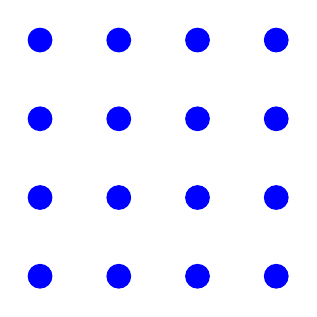
\begin{tikzpicture}
						\foreach \x in {1, 2, 3, 4} {
								\foreach \y in {1, 2, 3, 4} {
										\filldraw[blue] (\x, \y) circle(0.15);
									}
							}
					\end{tikzpicture}
				\end{center}
				\begin{choices}
					\choice Gas
					\choice Sólido
					\choice Líquido
					\choice Plasma
				\end{choices}

				\part ¿Qué sucede con las partículas de una sustancia al aumentar su temperatura?
				\begin{choices}
					\choice Se acercan más entre sí
					\choice Pierden energía
					\choice Aumentan su energía cinética
					\choice Se transforman en sólido
				\end{choices}

				\part El agua en forma de vapor se encuentra en el estado:
				\begin{choices}
					\choice Sólido
					\choice Líquido
					\choice Gas
					\choice Plasma
				\end{choices}

				\part ¿Cómo se llama el proceso mediante el cual un sólido pasa directamente a gas?
				\begin{choices}
					\choice Condensación
					\choice Sublimación
					\choice Evaporación
					\choice Fusión
				\end{choices}

				\part Observa el diagrama y responde: ¿Qué estado de la materia tiene partículas con mayor energía cinética?
				\begin{center}
					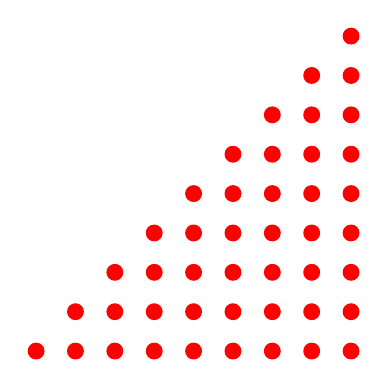
\begin{tikzpicture}
						\foreach \x in {1, 2, ..., 10} {
								\foreach \y in {1, 2, ..., 10} {
										\ifnum\x>\y
											\filldraw[red] (\x * 0.5, \y * 0.5) circle(0.1);
										\fi
									}
							}
					\end{tikzpicture}
				\end{center}
				\begin{choices}
					\choice Sólido
					\choice Líquido
					\choice Gas
					\choice Plasma
				\end{choices}

				\part El término "energía cinética" se refiere a:
				\begin{choices}
					\choice La energía almacenada en las partículas
					\choice La energía del movimiento de las partículas
					\choice La energía potencial de las partículas
					\choice La energía total de un objeto en reposo
				\end{choices}

			\end{parts}
		\end{multicols}
	}

	\questionboxed[6]{Relaciona los conceptos de la columna izquierda con su descripción en la columna derecha:

		\begin{multicols}{2}
			\begin{parts}
				\part Sólido
				\part Líquido
				\part Gas
				\part Plasma
				\part Sublimación
				\part Condensación
				\part Fusión
				\part Vaporización
				\part Energía Cinética
				\part Difusión
				\part Punto de ebullición
				\part Cambio físico
				\part Evaporación
				\part Condensación
				\part Densidad
			\end{parts}

			\columnbreak

			\begin{choices}
				\choice Cambio de sólido a líquido
				\choice Estado con partículas muy juntas y organizadas
				\choice Cambio de líquido a gas
				\choice Propiedad de movimiento de las partículas
				\choice Partículas en estado ionizado
				\choice Cambio directo de sólido a gas
				\choice Estado con partículas separadas y desordenadas
				\choice Movimiento de partículas de mayor concentración a menor
				\choice Cambio de gas a líquido
				\choice Estado fluido sin forma fija pero con volumen definido
				\choice Relación entre masa y volumen
				\choice Cambio en el que no se altera la composición
				\choice Temperatura en la que hierve una sustancia
				\choice Proceso de cambio líquido a gas a temperatura ambiente
				\choice Cambio de gas a líquido
			\end{choices}
		\end{multicols}
	}



	\questionboxed[10]{Observa el siguiente esquema y completa los espacios en blanco con los nombres de los procesos:
		\begin{center}
			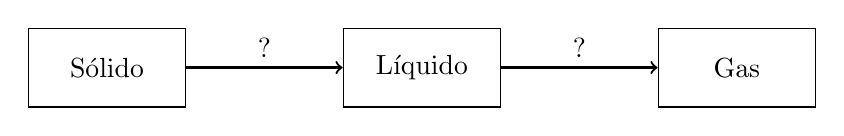
\begin{tikzpicture}
				% Sólido
				\node[draw, rectangle, minimum width=2cm, minimum height=1cm] (solid) at (0,0) {Sólido};
				% Líquido
				\node[draw, rectangle, minimum width=2cm, minimum height=1cm] (liquid) at (4,0) {Líquido};
				% Gas
				\node[draw, rectangle, minimum width=2cm, minimum height=1cm] (gas) at (8,0) {Gas};
				% Flechas
				\draw[->, thick] (solid) -- node[above] {?} (liquid);
				\draw[->, thick] (liquid) -- node[above] {?} (gas);
			\end{tikzpicture}
		\end{center}
	}

	% % Sólido - ejemplo 1
	% \begin{figure}[h]
	% 	\centering
	% 	\begin{tikzpicture}
	% 		\foreach \x in {0,1,2,3} {
	% 				\foreach \y in {0,1,2,3} {
	% 						\fill[blue] (\x,\y) circle (0.15);
	% 					}
	% 			}
	% 	\end{tikzpicture}
	% 	\caption{Sólido: partículas ordenadas y muy juntas}
	% \end{figure}

	% % Sólido - ejemplo 2
	% \begin{figure}[h]
	% 	\centering
	% 	\begin{tikzpicture}
	% 		\foreach \x in {0,1,2,3} {
	% 				\foreach \y in {0,1,2,3} {
	% 						\fill[red] (\x+0.1*\x,\y+0.1*\y) circle (0.15);
	% 					}
	% 			}
	% 	\end{tikzpicture}
	% 	\caption{Sólido: partículas compactas y organizadas con leve desplazamiento}
	% \end{figure}

	% % Líquido - ejemplo 1
	% \begin{figure}[h]
	% 	\centering
	% 	\begin{tikzpicture}
	% 		\foreach \x in {0,1,2,3} {
	% 				\foreach \y in {0,1,2,3} {
	% 						\fill[cyan] (\x + 0.5*rand, \y + 0.2*rand) circle (0.15);
	% 					}
	% 			}
	% 	\end{tikzpicture}
	% 	\caption{Líquido: partículas cercanas pero menos organizadas}
	% \end{figure}

	% % Líquido - ejemplo 2
	% \begin{figure}[h]
	% 	\centering
	% 	\begin{tikzpicture}
	% 		\foreach \x in {0,1,2,3} {
	% 				\foreach \y in {0,1,2} {
	% 						\fill[teal] (\x+0.4*rand, \y+0.6*rand) circle (0.15);
	% 					}
	% 			}
	% 	\end{tikzpicture}
	% 	\caption{Líquido: partículas con mayor desorden}
	% \end{figure}

	% % Gas - ejemplo 1
	% \begin{figure}[h]
	% 	\centering
	% 	\begin{tikzpicture}
	% 		\foreach \x in {0,1,2,3,4} {
	% 				\foreach \y in {0,1,2,3,4} {
	% 						\fill[orange] (\x + rand, \y + rand) circle (0.15);
	% 					}
	% 			}
	% 	\end{tikzpicture}
	% 	\caption{Gas: partículas dispersas y muy desordenadas}
	% \end{figure}

	% % Gas - ejemplo 2
	% \begin{figure}[h]
	% 	\centering
	% 	\begin{tikzpicture}
	% 		\foreach \x in {1,2,3,4,5} {
	% 				\foreach \y in {1,2,3} {
	% 						\fill[yellow] (\x+1.5*rand,\y+rand) circle (0.1);
	% 					}
	% 			}
	% 	\end{tikzpicture}
	% 	\caption{Gas: partículas muy separadas y sin orden}
	% \end{figure}

	% % Plasma - ejemplo 1
	% \begin{figure}[h]
	% 	\centering
	% 	\begin{tikzpicture}
	% 		\foreach \x in {1,2,3,4} {
	% 				\foreach \y in {1,2,3} {
	% 						\fill[red] (\x + rand,\y + rand) circle (0.1);
	% 						\fill[white] (\x + rand/2, \y + rand/2) circle (0.05);
	% 					}
	% 			}
	% 	\end{tikzpicture}
	% 	\caption{Plasma: partículas muy energéticas y aleatorias}
	% \end{figure}

	% % Plasma - ejemplo 2
	% \begin{figure}[h]
	% 	\centering
	% 	\begin{tikzpicture}
	% 		\foreach \x in {0,1,2,3,4} {
	% 				\foreach \y in {0,1,2,3} {
	% 						\fill[magenta] (\x+0.5*rand,\y+rand) circle (0.15);
	% 						\fill[white] (\x+0.5*rand/2, \y+0.5*rand) circle (0.05);
	% 					}
	% 			}
	% 	\end{tikzpicture}
	% 	\caption{Plasma: partículas con gran energía y electrones libres}
	% \end{figure}

	% % Sólido - ejemplo en recipiente
	% \begin{figure}[h]
	% 	\centering
	% 	\begin{tikzpicture}
	% 		% Recipiente
	% 		\draw[thick] (0,0) rectangle (4,3);
	% 		% Partículas sólidas organizadas
	% 		\foreach \x in {0.5,1.5,2.5,3.5} {
	% 				\foreach \y in {0.5,1.5,2.5} {
	% 						\fill[blue] (\x,\y) circle (0.15);
	% 					}
	% 			}
	% 	\end{tikzpicture}
	% 	\caption{Sólido en un recipiente: partículas organizadas y compactas}
	% \end{figure}

	% % Líquido - ejemplo en recipiente
	% \begin{figure}[h]
	% 	\centering
	% 	\begin{tikzpicture}
	% 		% Recipiente
	% 		\draw[thick] (0,0) rectangle (4,3);
	% 		% Superficie del líquido
	% 		\draw[thick, blue] (0,1.5) -- (4,1.5);
	% 		% Partículas líquidas
	% 		\foreach \x in {0.3,0.9,1.5,2.1,2.7,3.3} {
	% 				\foreach \y in {0.3,0.9,1.2} {
	% 						\fill[cyan] (\x,\y+0.5) circle (0.15);
	% 					}
	% 			}
	% 	\end{tikzpicture}
	% 	\caption{Líquido en un recipiente: partículas cercanas y menos organizadas}
	% \end{figure}

	% % Gas - ejemplo en recipiente
	% \begin{figure}[h]
	% 	\centering
	% 	\begin{tikzpicture}
	% 		% Recipiente
	% 		\draw[thick] (0,0) rectangle (4,3);
	% 		% Partículas gaseosas dispersas
	% 		\foreach \x in {0.5,1.5,2.5,3.5} {
	% 				\foreach \y in {0.5,1.5,2.5} {
	% 						\fill[orange] (\x+0.5*rand,\y+0.5*rand) circle (0.1);
	% 					}
	% 			}
	% 	\end{tikzpicture}
	% 	\caption{Gas en un recipiente: partículas dispersas y desordenadas}
	% \end{figure}

	% % Plasma - ejemplo en recipiente
	% \begin{figure}[h]
	% 	\centering
	% 	\begin{tikzpicture}
	% 		% Recipiente
	% 		\draw[thick] (0,0) rectangle (4,3);
	% 		% Partículas de plasma con electrones libres
	% 		\foreach \x in {0.5,1.5,2.5,3.5} {
	% 				\foreach \y in {0.5,1.5,2.5} {
	% 						\fill[red] (\x+0.5*rand,\y+0.5*rand) circle (0.12);
	% 						\fill[white] (\x+0.5*rand,\y+0.5*rand) circle (0.05);
	% 					}
	% 			}
	% 	\end{tikzpicture}
	% 	\caption{Plasma en un recipiente: partículas muy energéticas y electrones libres}
	% \end{figure}

	% % Ejemplo 1: Líquido con partículas cercanas en una capa densa
	% \begin{figure}[h]
	% 	\centering
	% 	\begin{tikzpicture}
	% 		% Recipiente
	% 		\draw[thick] (0,0) rectangle (4,3);
	% 		% Superficie ondulada del líquido
	% 		\draw[thick, blue] (0,1.2) to[out=10,in=170] (1,1.3)
	% 		to[out=10,in=170] (2,1.2)
	% 		to[out=10,in=170] (3,1.3)
	% 		to[out=10,in=170] (4,1.2);
	% 		% Partículas de líquido cercanas pero con cierto desorden
	% 		\foreach \x in {0.4,0.8,1.2,1.6,2.0,2.4,2.8,3.2,3.6} {
	% 				\foreach \y in {0.3,0.7,1.1} {
	% 						\fill[cyan] (\x+rand*0.2,\y) circle (0.15);
	% 					}
	% 			}
	% 	\end{tikzpicture}
	% 	\caption{Líquido en recipiente: partículas con organización aleatoria y superficie ondulada}
	% \end{figure}

	% % Ejemplo 2: Líquido con partículas en varias capas y con mayor desorden
	% \begin{figure}[h]
	% 	\centering
	% 	\begin{tikzpicture}
	% 		% Recipiente
	% 		\draw[thick] (0,0) rectangle (4,3);
	% 		% Superficie ondulada del líquido
	% 		\draw[thick, blue] (0,1.5) to[out=20,in=160] (1,1.3)
	% 		to[out=-20,in=160] (2,1.4)
	% 		to[out=20,in=160] (3,1.2)
	% 		to[out=-20,in=160] (4,1.5);
	% 		% Partículas de líquido en varias capas con mayor separación
	% 		\foreach \x in {0.3,0.9,1.5,2.1,2.7,3.3} {
	% 				\foreach \y in {0.3,0.8,1.2} {
	% 						\fill[teal] (\x+rand*0.3,\y+rand*0.2) circle (0.15);
	% 					}
	% 			}
	% 	\end{tikzpicture}
	% 	\caption{Líquido en recipiente: partículas con más desorden en varias capas}
	% \end{figure}

	% % Ejemplo 3: Líquido con partículas en disposición semicircular para simular flujo
	% \begin{figure}[h]
	% 	\centering
	% 	\begin{tikzpicture}
	% 		% Recipiente
	% 		\draw[thick] (0,0) rectangle (4,3);
	% 		% Superficie ondulada del líquido
	% 		\draw[thick, blue] (0,1.8) to[out=20,in=160] (1,1.6)
	% 		to[out=-20,in=160] (2,1.7)
	% 		to[out=20,in=160] (3,1.5)
	% 		to[out=-20,in=160] (4,1.8);
	% 		% Partículas en patrón semicircular, para simular movimiento y flujo
	% 		\foreach \x in {0.5,1.0,1.5,2.0,2.5,3.0,3.5} {
	% 				\fill[cyan] (\x,1.0 + 0.5*rand) circle (0.15);
	% 			}
	% 		\foreach \x in {0.7,1.2,1.7,2.2,2.7,3.2} {
	% 				\fill[cyan] (\x,0.6 + 0.5*rand) circle (0.15);
	% 			}
	% 	\end{tikzpicture}
	% 	\caption{Líquido en recipiente: partículas en un patrón semicircular para simular flujo}
	% \end{figure}

	% % Ejemplo 4: Líquido con partículas flotando parcialmente para simular inestabilidad
	% \begin{figure}[h]
	% 	\centering
	% 	\begin{tikzpicture}
	% 		% Recipiente
	% 		\draw[thick] (0,0) rectangle (4,3);
	% 		% Superficie ondulada del líquido
	% 		\draw[thick, blue] (0,1.3) to[out=15,in=165] (1,1.4)
	% 		to[out=-15,in=165] (2,1.3)
	% 		to[out=15,in=165] (3,1.4)
	% 		to[out=-15,in=165] (4,1.3);
	% 		% Partículas con algunas en la superficie y otras más bajas
	% 		\foreach \x in {0.3,0.9,1.5,2.1,2.7,3.3} {
	% 				\foreach \y in {0.3,0.7,1.0} {
	% 						\fill[cyan] (\x+rand*0.3,\y+0.5*rand) circle (0.15);
	% 					}
	% 			}
	% 	\end{tikzpicture}
	% 	\caption{Líquido en recipiente: partículas con algunas flotando en la superficie para simular inestabilidad}
	% \end{figure}


	% % Ejemplo Sólido 1: Partículas ordenadas en una cuadrícula
	% \begin{figure}[h]
	% 	\centering
	% 	\begin{tikzpicture}
	% 		\draw[thick] (0,0) rectangle (4,3);
	% 		\foreach \x in {0.5,1.5,2.5,3.5} {
	% 				\foreach \y in {0.5,1.5,2.5} {
	% 						\fill[blue] (\x,\y) circle (0.15);
	% 					}
	% 			}
	% 	\end{tikzpicture}
	% 	\caption{Sólido: Partículas ordenadas en cuadrícula.}
	% \end{figure}

	% % Ejemplo Sólido 2: Disposición hexagonal
	% \begin{figure}[h]
	% 	\centering
	% 	\begin{tikzpicture}
	% 		\draw[thick] (0,0) rectangle (4,3);
	% 		\foreach \x in {0.5,1.2,1.9,2.6,3.3} {
	% 				\foreach \y in {0.5,1.0,1.5,2.0,2.5} {
	% 						\fill[blue] (\x,\y) circle (0.15);
	% 					}
	% 			}
	% 	\end{tikzpicture}
	% 	\caption{Sólido: Partículas en disposición hexagonal.}
	% \end{figure}

	% % Ejemplo Sólido 3: Estructura escalonada
	% \begin{figure}[h]
	% 	\centering
	% 	\begin{tikzpicture}
	% 		\draw[thick] (0,0) rectangle (4,3);
	% 		\foreach \x in {0.5,1.5,2.5,3.5} {
	% 				\foreach \y in {0.7,1.7,2.7} {
	% 						\fill[red] (\x,\y) circle (0.15);
	% 					}
	% 			}
	% 	\end{tikzpicture}
	% 	\caption{Sólido: Estructura escalonada.}
	% \end{figure}

	% % Puedes continuar de esta forma para agregar más ejemplos de sólidos con variaciones en colores y posiciones

	% % ----- Estados de Agregación: Líquido -----
	% \subsection*{Líquido}

	% % Ejemplo Líquido 1: Partículas distribuidas aleatoriamente
	% \begin{figure}[h]
	% 	\centering
	% 	\begin{tikzpicture}
	% 		\draw[thick] (0,0) rectangle (4,3);
	% 		\draw[thick, blue] (0,1.2) -- (4,1.2);
	% 		\foreach \x in {0.3,0.9,1.5,2.1,2.7,3.3} {
	% 				\foreach \y in {0.3,0.9} {
	% 						\fill[cyan] (\x + 0.2*rand, \y + 0.2*rand) circle (0.15);
	% 					}
	% 			}
	% 	\end{tikzpicture}
	% 	\caption{Líquido: Partículas distribuidas de forma aleatoria.}
	% \end{figure}

	% % Ejemplo Líquido 2: Partículas densas en la parte inferior
	% \begin{figure}[h]
	% 	\centering
	% 	\begin{tikzpicture}
	% 		\draw[thick] (0,0) rectangle (4,3);
	% 		\draw[thick, blue] (0,1.4) to[out=20,in=160] (4,1.4);
	% 		\foreach \x in {0.4,1.2,2.0,2.8,3.6} {
	% 				\foreach \y in {0.4,0.8,1.2} {
	% 						\fill[cyan] (\x+0.2*rand,\y) circle (0.15);
	% 					}
	% 			}
	% 	\end{tikzpicture}
	% 	\caption{Líquido: Partículas densas en el fondo con leve movimiento.}
	% \end{figure}

	% % Puedes continuar de esta forma para agregar más ejemplos de líquidos con variaciones de patrones

	% % ----- Estados de Agregación: Gas -----
	% \subsection*{Gas}

	% % Ejemplo Gas 1: Partículas dispersas y distribuidas
	% \begin{figure}[h]
	% 	\centering
	% 	\begin{tikzpicture}
	% 		\draw[thick] (0,0) rectangle (4,3);
	% 		\foreach \x in {0.5,1.5,2.5,3.5} {
	% 				\foreach \y in {0.5,1.5,2.5} {
	% 						\fill[orange] (\x + 0.5*rand, \y + 0.5*rand) circle (0.1);
	% 					}
	% 			}
	% 	\end{tikzpicture}
	% 	\caption{Gas: Partículas dispersas.}
	% \end{figure}

	% % Ejemplo Gas 2: Partículas más densas en la parte superior
	% \begin{figure}[h]
	% 	\centering
	% 	\begin{tikzpicture}
	% 		\draw[thick] (0,0) rectangle (4,3);
	% 		\foreach \x in {0.5,1.5,2.5,3.5} {
	% 				\foreach \y in {1.5,2.0,2.5} {
	% 						\fill[orange] (\x + rand,\y + rand) circle (0.1);
	% 					}
	% 			}
	% 	\end{tikzpicture}
	% 	\caption{Gas: Partículas más concentradas en la parte superior.}
	% \end{figure}

	% % Ejemplo Sólido 1: Cuadrícula uniforme
	% \begin{figure}[h]
	% 	\centering
	% 	\begin{tikzpicture}
	% 		\draw[thick] (0,0) rectangle (4,3);
	% 		\foreach \x in {0.5,1.5,2.5,3.5} {
	% 				\foreach \y in {0.5,1.5,2.5} {
	% 						\fill[blue] (\x,\y) circle (0.15);
	% 					}
	% 			}
	% 	\end{tikzpicture}
	% 	\caption{Sólido 1: Cuadrícula uniforme.}
	% \end{figure}

	% % Ejemplo Sólido 2: Patrón hexagonal
	% \begin{figure}[h]
	% 	\centering
	% 	\begin{tikzpicture}
	% 		\draw[thick] (0,0) rectangle (4,3);
	% 		\foreach \x in {0.5,1.2,1.9,2.6,3.3} {
	% 				\foreach \y in {0.5,1.0,1.5,2.0,2.5} {
	% 						\fill[blue] (\x,\y) circle (0.15);
	% 					}
	% 			}
	% 	\end{tikzpicture}
	% 	\caption{Sólido 2: Patrón hexagonal.}
	% \end{figure}

	% % Ejemplo Sólido 3: Orden en filas con pequeñas separaciones
	% \begin{figure}[h]
	% 	\centering
	% 	\begin{tikzpicture}
	% 		\draw[thick] (0,0) rectangle (4,3);
	% 		\foreach \x in {0.6,1.2,1.8,2.4,3.0,3.6} {
	% 				\foreach \y in {0.6,1.2,1.8,2.4} {
	% 						\fill[red] (\x,\y) circle (0.15);
	% 					}
	% 			}
	% 	\end{tikzpicture}
	% 	\caption{Sólido 3: Filas con pequeñas separaciones.}
	% \end{figure}

	% % (Agrega más ejemplos similares de sólidos variando los patrones, colores y disposiciones)

	% \section*{Ejemplos de Líquidos}

	% % Ejemplo Líquido 1: Partículas dispersas con superficie ondulada
	% \begin{figure}[h]
	% 	\centering
	% 	\begin{tikzpicture}
	% 		\draw[thick] (0,0) rectangle (4,3);
	% 		\draw[thick, blue] (0,1.4) to[out=20,in=160] (4,1.4);
	% 		\foreach \x in {0.4,1.0,1.6,2.2,2.8,3.4} {
	% 				\foreach \y in {0.4,0.8,1.2} {
	% 						\fill[cyan] (\x+rand*0.2,\y) circle (0.15);
	% 					}
	% 			}
	% 	\end{tikzpicture}
	% 	\caption{Líquido 1: Partículas dispersas con superficie ondulada.}
	% \end{figure}

	% % Ejemplo Líquido 2: Líquido con partículas agrupadas en el fondo
	% \begin{figure}[h]
	% 	\centering
	% 	\begin{tikzpicture}
	% 		\draw[thick] (0,0) rectangle (4,3);
	% 		\draw[thick, blue] (0,1.2) -- (4,1.2);
	% 		\foreach \x in {0.4,0.8,1.2,1.6,2.0,2.4,2.8,3.2,3.6} {
	% 				\foreach \y in {0.4,0.8} {
	% 						\fill[teal] (\x+rand*0.3,\y) circle (0.15);
	% 					}
	% 			}
	% 	\end{tikzpicture}
	% 	\caption{Líquido 2: Líquido con partículas agrupadas en el fondo.}
	% \end{figure}

	% % (Agrega más ejemplos similares de líquidos variando las distribuciones y formas de la superficie)

	% \section*{Ejemplos de Gases}

	% % Ejemplo Gas 1: Partículas dispersas en todo el recipiente
	% \begin{figure}[h]
	% 	\centering
	% 	\begin{tikzpicture}
	% 		\draw[thick] (0,0) rectangle (4,3);
	% 		\foreach \x in {0.5,1.0,1.5,2.0,2.5,3.0,3.5} {
	% 				\foreach \y in {0.5,1.0,1.5,2.0,2.5} {
	% 						\fill[orange] (\x + rand,\y + rand) circle (0.1);
	% 					}
	% 			}
	% 	\end{tikzpicture}
	% 	\caption{Gas 1: Partículas dispersas en todo el recipiente.}
	% \end{figure}

	% % Ejemplo Gas 2: Mayor densidad de partículas en la parte superior
	% \begin{figure}[h]
	% 	\centering
	% 	\begin{tikzpicture}
	% 		\draw[thick] (0,0) rectangle (4,3);
	% 		\foreach \x in {0.4,1.0,1.6,2.2,2.8,3.4} {
	% 				\foreach \y in {2.0,2.4,2.8} {
	% 						\fill[orange] (\x + rand,\y + rand) circle (0.1);
	% 					}
	% 			}
	% 	\end{tikzpicture}
	% 	\caption{Gas 2: Mayor densidad en la parte superior del recipiente.}
	% \end{figure}

\end{questions}
\end{document}